\section{PRFs from Hash functions}

\subsection{Other Hash based PRFs}
The Merkle Damg{\aa}rd construction from the previous section is a type of Prefix MAC (since the key is prepended to the message). Although the construction is a secure PRF in the random oracle model, we saw how it is susceptible to length extension attacks. Several alternatives have been proposed to counter these attacks. We use $\hash^f$ to represent the Merkle Damg{\aa}rd construction with $f$ as the underlying compression function.  

\paragraph{Suffix MAC:}
$\hash^f(M \Vert K)$ - The key is appended to the end instead of the beginning. Now, for a length extension attack to succeed, the adversary must find a collision for hash output of the message prefix until the key is added. To elaborate, if the adversary finds messages $M_0$ and $M_1$ such that $\hash^f(M_0) = \hash^f(M_1)$ by an offline collision attack, then it can break security for the overall construction without ever needing the key. To prove \PRF-security, therefore, we require that $\hash$ be collision resistant.


\paragraph{Envelope MAC:} $\hash^f(K_1 \Vert M \Vert K_2)$ - A key $K_1$ is prepended and another key $K_2$ is appended to the input. The \PRF-security proof is similar to the one before except now collision resistance is no longer required.

\paragraph{Nested MAC:}
$\hash^f(K_1 \Vert \hash^f(K_2 \Vert M))$ - The standard Prefix MAC construction is applied to the message twice with two \textit{independently} chosen keys $K_1$ and $K_2$.


\subsection{The HMAC Construction}

$\HMAC$, a widely used MAC in practice is a close variant of the nested MAC. For $\HMAC$, The keys $K_1$ and $K_2$ are no longer picked independently but rather derived from some base key $K$. The keys are computed as $K_1 = f(\IV, K \oplus \ipad)$ and $K_2 = f(\IV, K \oplus \opad)$ where $\ipad$ (inner pad) and $\opad$ (outer pad) are constants. The usage of a single base key rather than two allows $\HMAC$ to be built using existing SHA hash functions in a black-box way. Figure \ref{fig: HMAC construction} shows both a shortened and an extended version of the $\HMAC$ construction

\begin{figure}[h]
\centering
\subcaptionbox{%
    % 
    \label{fig:HMAC 1}
  }[0.3\linewidth] {
   \begin{tikzpicture}[scale=0.4]
            \begin{scope}[]
                \node [draw,trapezium,trapezium left angle=70,trapezium right angle=70,minimum height=0.75cm,thick,fill=orange!15,shift={(1.15,0)},rotate=-90] 
                {\begin{sideways}\Large $\hash$ \end{sideways}};
                \draw[->,thick] (0,0) node[left] {$K_1 \Vert M $} -- (1.9,0);
                \draw[->,thick] ++(4,0) -- ++(1.5,0) -- ++(0,-2.5);
            \end{scope}
            \begin{scope}[shift={(6.2,-3.25)}]
                \node [draw,trapezium,trapezium left angle=70,trapezium right angle=70,minimum height=0.75cm,thick,fill=orange!15,shift={(1.15,0)},rotate=-90] 
                {\begin{sideways}\Large $\hash$ \end{sideways}};
                \draw[->,thick] (0,0) node[left] {$K_2 \Vert h$} -- (1.9,0);
                \draw[->,thick] ++(4,0) -- ++(2,0) node[right] {$Y$};
            \end{scope}
        \end{tikzpicture}
    }
\hfill
\subcaptionbox{%
   % \label{fig:HMAC 2}
  }[0.5 \linewidth]
  { 
  \begin{tikzpicture}[scale=0.4]
            \begin{scope}[]
                \node [draw,trapezium,trapezium left angle=50,trapezium right angle=90,minimum height=0.5cm,thick,fill=orange!15,shift={(1.15,0.3)},rotate=-90] 
                {\begin{sideways}\Large$f$\end{sideways}};
                \draw[->,thick] ++(0.5,+3) node[above] {$K \oplus \ipad$} -- ++(0,-1) -- ++(1.7,0);
                \draw[->,thick] ++(0,0.5) node[left] {IV} -- ++(2.2,0);
            \end{scope}

            \begin{scope}[shift={(3.5,0)}]
                \node [draw,trapezium,trapezium left angle=50,trapezium right angle=90,minimum height=0.5cm,thick,fill=orange!15,shift={(1.15,0.3)},rotate=-90] 
                {\begin{sideways}\Large$f$\end{sideways}};
                \draw[->,thick] ++(0.5,+3) node[above] {$M_1$} -- ++(0,-1) -- ++(1.7,0);
                \draw[->,thick] ++(0,0.5) -- node[below] {$K_1$} ++(2.2,0);
            \end{scope}

            \begin{scope}[shift={(7,0)}]
                \node [draw,trapezium,trapezium left angle=50,trapezium right angle=90,minimum height=0.5cm,thick,fill=orange!15,shift={(1.15,0.3)},rotate=-90] 
                {\begin{sideways}\Large$f$\end{sideways}};
                \draw[->,thick] ++(0.5,+3) node[above] {$M_2$} -- ++(0,-1) -- ++(1.7,0);
                \draw[->,thick] ++(0,0.5) --  ++(2.2,0);
            \end{scope}
            
            \begin{scope}[shift={(7,-6)}]
                \node [draw,trapezium,trapezium left angle=50,trapezium right angle=90,minimum height=0.5cm,thick,fill=orange!15,shift={(1.15,0.3)},rotate=-90] 
                {\begin{sideways}\Large$f$\end{sideways}};
                \draw[->,thick] ++(0.5,+3) node[above] {$K \oplus \opad$} -- ++(0,-1) -- ++(1.7,0);
                \draw[->,thick] ++(0,0.5) node[left] {IV} --  ++(2.2,0);
            \end{scope}
            
            \begin{scope}[shift={(10.5,-6)}]
                \node [draw,trapezium,trapezium left angle=50,trapezium right angle=90,minimum height=0.5cm,thick,fill=orange!15,shift={(1.15,0.3)},rotate=-90] 
                {\begin{sideways}\Large$f$\end{sideways}};
                \draw[->,thick] ++(0,+6.4) -- ++(0.5, 0) -- ++(0,-4.4) -- ++(1.7,0);
                \draw[->,thick] ++(0,0.5) -- node[below] {$K_2$} ++(2.2,0);
                \draw[->,thick] ++(3.6,0.5) -- ++(2,0) node[right] {$Y$};
            \end{scope}
        \end{tikzpicture} 
    }
    \caption{HMAC construction} \label{fig: HMAC construction}
\end{figure}


\subsection{Analysis of HMAC}
To analyze the PRF security of the $\HMAC$ construction, we can first prove security under the assumption that the hash function is a random oracle $\Horacle$. Notice that now the dependence of keys $K_1$ and $K_2$ no longer matters; the proof will apply for the regular Nested MAC. We leave the formal proof to the reader as \ref{Exercise 1} 

While security in the RO model is a good sanity check, it is usually not sufficient by itself. Attacks on real world hash based constructions can take advantage of the underlying structure to break security.
This naturally begs the question: What assumptions are reasonable to show security of real world constructions? We argue that it might be reasonable to assume that the underlying compression function $f$ is a good PRF to prove security. We defer further details till the next section.

What does it mean exactly for $f$ to be a ``good'' PRF here? A strawman answer would be to make sure that $f$ is secure under the standard PRF security game. Unfortunately, the standard PRF game provides no room for an adversary to use the output under a related key to distinguish between the real and ideal worlds. Recall that for $\HMAC$, $K_1$ and $K_2$ are derived from a single key $K$. Even then, ideally an adversary should not be able to correlate the outputs of $f$ under the two keys. Intuitively, we want to ask whether $K_1$ and $K_2$ are indistinguishable from random bit strings \textit{even when} the adversary can see outputs under related keys. 
We resolve this mismatch by constructing a slightly different game $\RKAPRF$ (Figure \ref{fig:RKA}). Statements modified from the original PRF game are colored blue. Suppose $f$ takes as input a $d$ bit key and an $n$ bit message and compresses them to a single $n$ bit output. That is, $f: \bits^n \times \bits^d \to \bits^n$. The game is now parametrized by a set of functions $\Phi$ and the adversary can now query the oracle using a related key $\phi(K)$ for any $\phi \in \Phi$. The adversarial advantage for the $\RKAPRF$ game is defined in the standard way:
\[
\AdvRKAPRF{f, \Phi}{\advA} = 
\left| 
    \Pr[\LRKAPRFIdeal^\advA_{f,\Phi} \Rightarrow 1] 
    - \Pr[\LRKAPRFReal^\advA_{f,\Phi} \Rightarrow 1]
\right|
\]


\begin{figure}[h]
\centering
\hfpagess{.15}{.25}{
    \underline{$\LRKAPRFIdeal^\advA_{f, \modify{\Phi}}$}\\[1pt]
    $K \getsr \bits^d$\\
    $b' \getsr \advA^{\FnOracle}$\\
    Ret $b'$\medskip

    \underline{$\FnOracle(\modify{\phi}, X)$}\\
    \modify{If $\phi \in \Phi$ then}\\
    \modify{\myInd Ret $\bot$}\\
    Ret $f(X,\modify{\phi(K)})$\medskip
}
{
    \underline{$\LRKAPRFReal^\advA_{f, \modify{\Phi}}$}\\[1pt]
    $K \getsr \bits^d$\\
    $\rho \getsr \Func(\modify{\bits^n \times \bits^d},n)$\\
    $b' \getsr \advA^{\FnOracle}$\\
    Ret $b'$\medskip

    \underline{$\FnOracle(\modify{\phi}, X)$}\\
    \modify{If $\phi \in \Phi$ then}\\
    \modify{\myInd Ret $\bot$}\\
    Ret $\rho(X \modify{, \phi(K)})$\medskip
}
\caption{Related Key Attack Game} \label{fig:RKA}
\end{figure}



We note that this game modification is far more general than what might be needed for HMAC security. For our application, it is reasonable to restrict $\Phi$ to just $\phi_{\ipad}$ and $\phi_{\opad}$ where $\phi_{\ipad}(K) = K \oplus \ipad$ and $\phi_{\opad}(K) = K \oplus \opad$ and then ask whether $f$ is \RKAPRF secure. Choosing such an $f$ function would imply that $K_1$ and $K_2$ are indistinguishable from random bit strings. 

Suppose now that we have ensured that the compression function $f$ used in HMAC is \RKAPRF secure. We still need to show that the overall construction is \PRF-secure. 

\begin{lemma}
(Informal) If $f$ is $\RKAPRF$-secure and the iterated keyed hash function $\hash$ is collision resistant then the $\HMAC$ construction is $\PRF$-secure
\end{lemma}
\begin{proofsketch}
If $f$ is $\RKAPRF$-secure, then the keys $K_1$ and $K_2$ are indistinguishable from random bit strings even for adversaries that use outputs from related key functions $\phi_{\ipad}$ and $\phi_{\opad}$. Now, we have seen that the composition of a collision resistant function and a secure PRF is a secure PRF. Therefore, we can conclude that $\HMAC$ is PRF-secure
\end{proofsketch}

\noindent Some subtleties like block padding have been ignored in the above sketch. A detailed proof can be found in \cite{Bellare1996}. A stronger result that does not rely on the collision resistance of $\hash$ (but instead on some weaker assumptions) is proved in \cite{Bellare2006}

\subsection{The Indifferentiability Framework}
We've seen that security analysis in the RO model is insufficient justification for instantiating constructions with real hash functions. Understanding security of real world constructions would be a lot easier if we had a general framework that accounted for structure-abusing attacks on hash functions. Coron et al. \cite{Coron2005} suggest use of the Indifferentiability franework introduced by Maurer et al. \cite{Maurer2004} in the context of hash functions. At a high level, we model the inner compression function $f$ itself as a random oracle for fixed-length inputs and attempt to prove that the overall construction is indistinguishable from a random oracle. Indifferentiability from a random oracle can be considered approximately as secure as a random oracle. 

Figure \ref{fig:Indiff Diagram} shows the schematic representation of the framework. As usual, $\advD$ tries to distinguish between the ideal world (with a random oracle) and the real world (with the construction $\hash^f$). In the real world, $\advD$ also gets access to the underlying function $f$. In the ideal world, since $\RO$ does not depend on $f$, a simulator $\simoracle$ tries to simulate the function $f$. $\advD$ gets access to this simulator in the ideal world. Figure \ref{fig:Indiff Game} describes the $\INDIFF$ game in detail.


\begin{figure}[h]
\centering
\subcaptionbox{%
    Diagram \label{fig:Indiff Diagram}
    \label{fig:NMAC}
  }[0.5\linewidth] {
    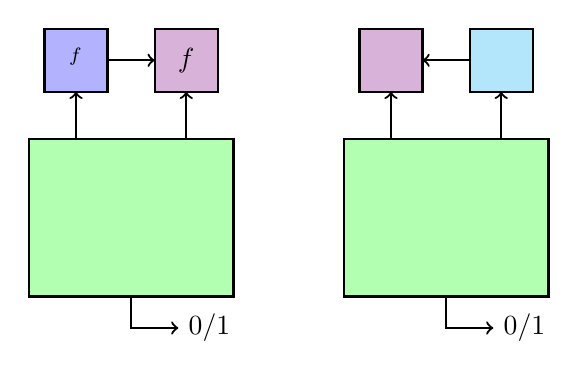
\begin{tikzpicture}[scale=0.4]
        \begin{scope}[]
            \draw[fill=blue!30,thick] (0.5,6.5) rectangle ++(2,2) node[pos=.5] {$\hash^f$};
            \draw[fill=violet!30,thick] (4,6.5) rectangle ++(2,2) node[pos=.5] {$f$};
            \draw[fill=green!30,thick] (0,0) rectangle ++(6.5,5) node[pos=.5]  {$\advD$};
            
            \draw[->, thick] ++(2.5,7.5) -- ++(1.5,0);  % H to f
            \draw[->, thick] ++(1.5,5) -- ++(0,1.5);    % D to H
            \draw[->, thick] ++(5,5) -- ++(0,1.5);      % D to f
            
            \draw[->,thick] ++(3.25,0) -- ++(0,-1) -- ++(1.5,0) node[right] {0/1};
        \end{scope}
    
        \begin{scope}[shift={(10,0)}]
            \draw[fill=violet!30,thick] (0.5,6.5) rectangle ++(2,2) node[pos=.5] {$\RO$};
            \draw[fill=cyan!30,thick] (4,6.5) rectangle ++(2,2) node[pos=.5] {$\simoracle$};
            \draw[fill=green!30,thick] (0,0) rectangle ++(6.5,5) node[pos=.5]  {$\advD$};
            
            \draw[<-, thick] ++(2.5,7.5) -- ++(1.5,0);  % RO to Sim
            \draw[->, thick] ++(1.5,5) -- ++(0,1.5);    % D to RO
            \draw[->, thick] ++(5,5) -- ++(0,1.5);      % D to Sim
            
            \draw[->,thick] ++(3.25,0) -- ++(0,-1) -- ++(1.5,0) node[right] {0/1};
        \end{scope}
    
    \end{tikzpicture}
    }
\hfill
\subcaptionbox{%
   Game \label{fig:Indiff Game}
  }[0.4 \linewidth]
  { 
       \hfpagess{.15}{.15}{
            \underline{$\INDIFF1^\advD_{\hash, f}$}\\[1pt]
            $b' \getsr \advD^{\FnOracle, f}$\\
            Ret $b'$\medskip
        
            \underline{$\FnOracle(M)$}\\
            Ret $\hash^f(M)$\medskip
            
            \underline{$f(X)$}\\
            If $\ftable[X] = \bot$ then\\
            \myInd $\ftable[X] \getsr \bits^n$\\
            Ret $\ftable[X]$
        }
        {
            \underline{$\INDIFF0^\advD_{\Horacle, \simoracle}$}\\[1pt]
            $b' \getsr \advD^{\FnOracle, \simoracle}$\\
            Ret $b'$\medskip
        
            \underline{$\FnOracle(M)$}\\
            If $\Htable[M] = \bot$ then\\
            \myInd $\Htable[M] \getsr \bits^n$\\
            Ret $\Htable[M]$\\
            
            \underline{$\simoracle(X)$}\\
            Ret $\mathcal{S}^\FnOracle[X]$
        }
    }
    \caption{Indifferentiability from a Random Oracle} \label{fig:Indiff}
\end{figure}

\noindent We define a distinguisher $\advD$'s advantage in the $\INDIFF$ game as:
\[
\AdvINDIFF{\hash, f, \mathcal{S}}{\advD} = 
\left| 
    \Pr[\INDIFF1^\advD_{\hash,f} \Rightarrow 1] 
    - \Pr[\INDIFF0^\advD_{\Horacle,\mathcal{S}} \Rightarrow 1]
\right|
\]

\begin{wrapfigure}{r}{1.5in}
    \centering
    \fpage{.2}{
            \underline{$\textbf{adversary } \advD^{\FnOracle, O}$}\\[1pt]
            $m_1, m_2 \getsr \bits^d$\\
            $y_1 \gets \FnOracle(m_1)$\\
            $y_2 \gets O(y_1,  m_2)$\\
            $y'_2 \gets \FnOracle(m_1 \Vert m_2)$\\
            Ret $(y_2 = y'_2)$
    }
    \caption{MD adversary} \label{fig:Indiff distinguisher}
\end{wrapfigure}

\noindent First, we note that a good simulator $\simoracle$ for $f$ in the ideal world may not always exist. In fact, the Merkle Damg{\aa}rd construction is actually not indifferentiable from a random oracle. Consider the $\INDIFF$-adversary $\advD$ defined in Figure~\ref{fig:Indiff distinguisher}.
In the real world, the two outputs $y_2$ and $y'_2$ will always be equal. On the other hand, in the ideal world, the probability that $y_2$ and $y'_2$ are equal is just the probability that a randomly sampled $n$ bit string is equal to the $y_2$ output by the simulator; this is equal to $\frac{1}{2^n}$. Therefore, $\advD$ distinguishes between the real and ideal worlds with high probability.

Variations of the Merkle Damg{\aa}rd construction such as the Chopped MD or the Enveloped MD are often used in practice instead since they are indifferentiable from a random oracle

\bigskip
\noindent How is this indifferentiable framework useful? It's real power is seen through the following composition theorem which allows security analysis of a construction that uses the hash function $\hash^f$ for any arbitrary game $G$

\begin{theorem}
\label{thm: indiff composition}
\textbf{Indifferentiability Composition Theorem} \cite{Maurer2004}
For any security game $G$, construction $\hash^f$ and scheme $C$, if 
\begin{enumerate}
    \item $\hash^f$ is indifferentiable from a random oracle under the assumption that $f$ is a random oracle
    \item C is provably $G$-secure in the random oracle model
\end{enumerate}
then, $C$ is provably $G$-secure using $\hash^f$ under the assumption that $f$ is a random oracle

\end{theorem}


\begin{figure}[h]
    \centering
    
    \begin{tikzpicture}[scale=0.4]
\begin{scope}[]
    \draw[fill=blue!30,thick] (0.5,6.5) rectangle ++(2,2) node[pos=.5] {$\hash^f$};
    \draw[fill=violet!30,thick] (4,6.5) rectangle ++(2,2) node[pos=.5] {$f$};
    \draw[fill=green!30,thick] (0,0) rectangle ++(6.5,5);
    \draw[fill=gray!30] (0.5,0.25) rectangle ++(5.5,1.5) node[pos=.5] {$G$};
    \draw[fill=gray!30] (0.5,2.75) rectangle ++(2,2) node[pos=.5] {$C$};
    \draw[fill=red!30] (4,2.75) rectangle ++(2,2) node[pos=.5] {$\advA$};
    
    \draw[->, thick] ++(2.5,7.5) -- ++(1.5,0);      % H to f
    \draw[->, thick] ++(1.5,4.75) -- ++(0,1.75);    % C to H
    \draw[->, thick] ++(5,4.75) -- ++(0,1.75);      % A to f
    
    \draw[<->, thick] ++(2.5,3.75) -- ++(1.5,0);    % C to A
    \draw[->, thick] ++(1.5,1.75) -- ++(0,1);       % G to C
    \draw[->, thick] ++(5,1.75) -- ++(0,1);         % G to A

    \draw[->,thick] ++(3.25,0.25) -- ++(0,-1) -- ++(1.5,0) node[right] {0/1};

    \draw[<-, thick] ++(6.5,5) -- ++(1.25,1);
    \node[] at (8.25,6) {$\advD$};

\end{scope}

\begin{scope}[shift={(10,0)}]
    \draw[<-, thick] ++(0,5) -- ++(-1.25,1);

    \draw[fill=green!30,thick] (0,0) rectangle ++(6.5,5);
    \draw[fill=red!10] (3.75,2.5) rectangle ++(2.5, 6.25) node[right] {$\advB$};

    \draw[fill=violet!30,thick] (0.5,6.5) rectangle ++(2,2) node[pos=.5] {$\RO$};
    \draw[fill=cyan!30,thick] (4,6.5) rectangle ++(2,2) node[pos=.5] {$\simoracle$};

    \draw[fill=gray!30] (0.5,0.25) rectangle ++(5.5,1.5) node[pos=.5] {$G$};
    \draw[fill=gray!30] (0.5,2.75) rectangle ++(2,2) node[pos=.5] {$C$};
    \draw[fill=red!30] (4,2.75) rectangle ++(2,2) node[pos=.5] {$\advA$};
    
    \draw[<-, thick] ++(2.5,7.5) -- ++(1.5,0);  % Sim to RO
    \draw[->, thick] ++(1.5,4.75) -- ++(0,1.75);    % C to RO
    \draw[->, thick] ++(5,4.75) -- ++(0,1.75);      % A to Sim
    
    \draw[<->, thick] ++(2.5,3.75) -- ++(1.5,0);    % C to A
    \draw[->, thick] ++(1.5,1.75) -- ++(0,1);       % G to C
    \draw[->, thick] ++(5,1.75) -- ++(0,1);         % G to A
    
    \draw[->,thick] ++(3.25,0.25) -- ++(0,-1) -- ++(1.5,0) node[right] {0/1};
\end{scope}

\begin{scope}[shift={(20,0)}]

    \draw[fill=violet!30,thick] (0.5,6.5) rectangle ++(2,2) node[pos=.5] {$\RO$};
    \draw[fill=gray!30] (0.5,0.25) rectangle ++(5.5,1.5) node[pos=.5] {$G$};
    \draw[fill=gray!30] (0.5,2.75) rectangle ++(2,2) node[pos=.5] {$C$};
    \draw[fill=red!10] (4,2.75) rectangle ++(2,2) node[pos=.5] {$\advB$};
    
    \draw[<-, thick] ++(2.5,7.5) -- ++(2.5,0) --  ++(0,-2.75);      % B to RO
    \draw[->, thick] ++(1.5,4.75) -- ++(0,1.75);    % C to RO
    
    \draw[<->, thick] ++(2.5,3.75) -- ++(1.5,0);    % C to A
    \draw[->, thick] ++(1.5,1.75) -- ++(0,1);       % G to C
    \draw[->, thick] ++(5,1.75) -- ++(0,1);         % G to A
    
    \draw[->,thick] ++(3.25,0.25) -- ++(0,-1) -- ++(1.5,0) node[right] {0/1};
\end{scope}

\end{tikzpicture}
  
    \caption{Composition Theorem}
    \label{fig:indiff composition}
\end{figure}


\begin{proofsketch}
Suppose $C$ is $G$-secure in the random oracle model. We can split an adversary $\advB$ into two parts; the part ($\advA$) that interacts with the construction and the part ($\simoracle$) that handles calls to the RO. Now, consider the code of $C, \advA$ and $G$ as a single distinguisher $\advD$ for the $\INDIFF$ game. Since $\hash^f$ is indistinguishable from RO, $\advD$'s advantage for distinguishing between the real world (with $\hash^f, f$) and the ideal world (with $\RO, \simoracle$) is small. This means that the advantage of an adversary $\advA$ for game $G$ and construction $C$ using $\hash^f$ is small as well since otherwise we could construct $\advD$ as the code of $C, \advA$ and $G$ to win the $\INDIFF$ game.
We can now conclude that $C$ is $G$-secure using $\hash^f$.
\end{proofsketch}

A detailed proof can be found in \cite{Maurer2004}. The composition theorem allows for the security proofs to be modular. A construction that is secure in the random oracle model will also be secure in the standard model when instantiated using a hash function that is indifferentiable from RO. Therefore, it is now enough to prove security of the construction in the RO model to use it with a real hash function that has already been proven indifferentiable. This has led to ``indifferentiability from RO'' becoming a core requirement for modern hash function designs like SHA3. An important caveat to note however, is that the composition theorem may not apply to all games as shown by Ristenpart, Shacham and Shrimpton \cite{Ristenpart2011}. 



\subsection*{Exercises}
\begin{enumerate}[label=\textbf{Exercise \thesection.\arabic*}, wide=0pt]
    \item \label{Exercise 1} Prove $\PRF$-security of the HMAC construction under the assumption that the hash function is a random oracle.
\end{enumerate}
\setenumerate[1]{label=\arabic*.}
